\question[10] Las gráficas indican la tarifa de internet de dos compañías telefónicas.

\begin{figure}[H]
    \centering
    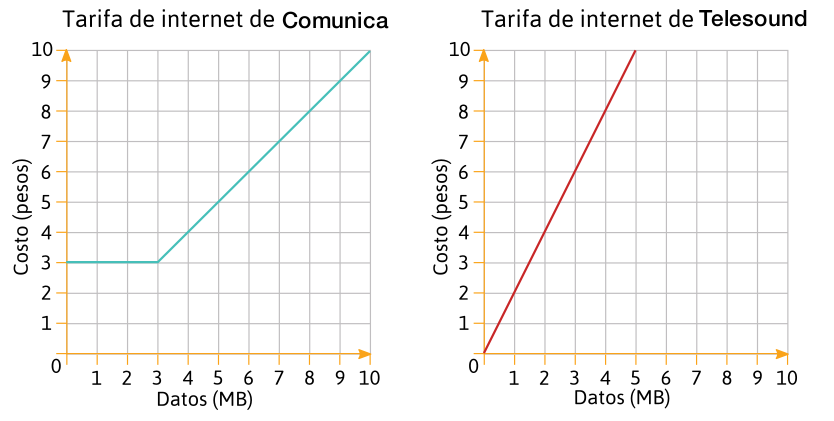
\includegraphics[width=0.45\textwidth]{../images/companias_telefon}
    \caption{}
    \label{fig:}
\end{figure}

\begin{parts}
    \part ¿Cuál de las dos compañías tiene una tarifa inicial de 3 pesos por los primeros 3 MB?
    \part ¿Cuál de las dos compañías ofrece la tarifa más alta después de los 3 MB?
    \part ¿En cuál de las dos compañías la relación entre el costo y la cantidad de datos es una variación proporcional?
    \part ¿Qué características de la gráfica representa una variación proporcional entre el costo y la cantidad de datos?
\end{parts}